\documentclass[a4paper, 11px]{article}

\usepackage[french]{babel}
\usepackage[utf8]{inputenc}
\usepackage{fancyhdr}
\usepackage{lastpage}
\usepackage{graphicx}
\usepackage{rotating}
\usepackage{textcomp}
\usepackage{xspace}
\usepackage[toc,page]{appendix}
\usepackage{array}
\usepackage{amssymb}
\usepackage{enumerate}
\usepackage{enumitem}
\usepackage{eso-pic}
\usepackage{hyperref}

% \usepackage{needspace}


%%%%%%
 
\usepackage{listings}

\lstset{
  morekeywords={},
  sensitive=f,
  morecomment=[l]--,
  morestring=[d]",
  showstringspaces=false,
  basicstyle=\small\ttfamily,
  keywordstyle=\bf\small,
  commentstyle=\itshape,
  stringstyle=\sf,
  extendedchars=true,
  columns=[c]fixed
}

% CI-DESSOUS: conversion des caractères accentués UTF-8 
% en caractères TeX dans les listings...
\lstset{
  literate=%
  {À}{{\`A}}1 {Â}{{\^A}}1 {Ç}{{\c{C}}}1%
  {à}{{\`a}}1 {â}{{\^a}}1 {ç}{{\c{c}}}1%
  {É}{{\'E}}1 {È}{{\`E}}1 {Ê}{{\^E}}1 {Ë}{{\"E}}1% 
  {é}{{\'e}}1 {è}{{\`e}}1 {ê}{{\^e}}1 {ë}{{\"e}}1%
  {Ï}{{\"I}}1 {Î}{{\^I}}1 {Ô}{{\^O}}1%
  {ï}{{\"i}}1 {î}{{\^i}}1 {ô}{{\^o}}1%
  {Ù}{{\`U}}1 {Û}{{\^U}}1 {Ü}{{\"U}}1%
  {ù}{{\`u}}1 {û}{{\^u}}1 {ü}{{\"u}}1%
}

%%%%%%%%%%
% TAILLE DES PAGES (A4 serré)

\setlength{\parindent}{1cm}
\setlength{\parskip}{1ex}
\setlength{\textwidth}{17cm}
\setlength{\textheight}{22,7cm}
\setlength{\oddsidemargin}{-.7cm}
\setlength{\evensidemargin}{-.7cm}


\renewcommand{\labelenumi}{\arabic{enumi}.} 
\renewcommand{\labelenumii}{\arabic{enumi}.\arabic{enumii}}
\renewcommand{\labelenumiii}{\arabic{enumi}.\arabic{enumii}.\arabic{enumiii}}

%%%%%%%%%%

\newcommand\BackgroundPic{
\put(0,0){
\parbox[b][\paperheight]{\paperwidth}{%
\vfill

\includegraphics[width=\paperwidth,height=\paperheight,
keepaspectratio]{background.jpg}%
\vfill
}}}
%%%%%%%

\begin{document}

\AddToShipoutPicture{\BackgroundPic}


\renewcommand{\appendixtocname}{Annexes}
\DeclareGraphicsExtensions{.pdf,.png,.jpg}

\begin{titlepage}
\setlength{\parindent}{0cm}

\begin{center}

% Upper part of the page
 \begin{figure}[!h]

\includegraphics[bb=-550 -10 -250 20, scale=0.7]{./logo.pdf}
\end{figure}
% logo.pdf: 612x792 pixel, 72dpi, 21.59x27.94 cm, bb=0 0 612 792


\vspace{4cm}
\rule{\linewidth}{.5pt}
\vspace{2mm}


\begin{center}
{\LARGE GRAND CERCLE MOBILE - GCM}

\vspace{1cm}


{\Huge \bf Document d'implantation}


\end{center}


\vspace{1cm}

%===================================================
\begin{center}
$ $\\
\large{ \textbf{Luiza CICONE - Jérémy KREIN - Jérémy LUQUET - Paul MAYER}}\\
\large{ \textbf{ISI - IF}}\\
\large{ \textbf{Tutrice : Gaëlle CALVARY}}
$ $\\
\end{center}
\rule{\linewidth}{.5pt}


\vfill

% Bottom of the page

{\large Mai 2012}

\end{center}
\end{titlepage}

\tableofcontents

\newpage

\section {Conception}
\subsection{Conception ergonomique}

%%%%%% Début DSE
\subsubsection{Cas d'utilisations}
\begin{figure}[h!]
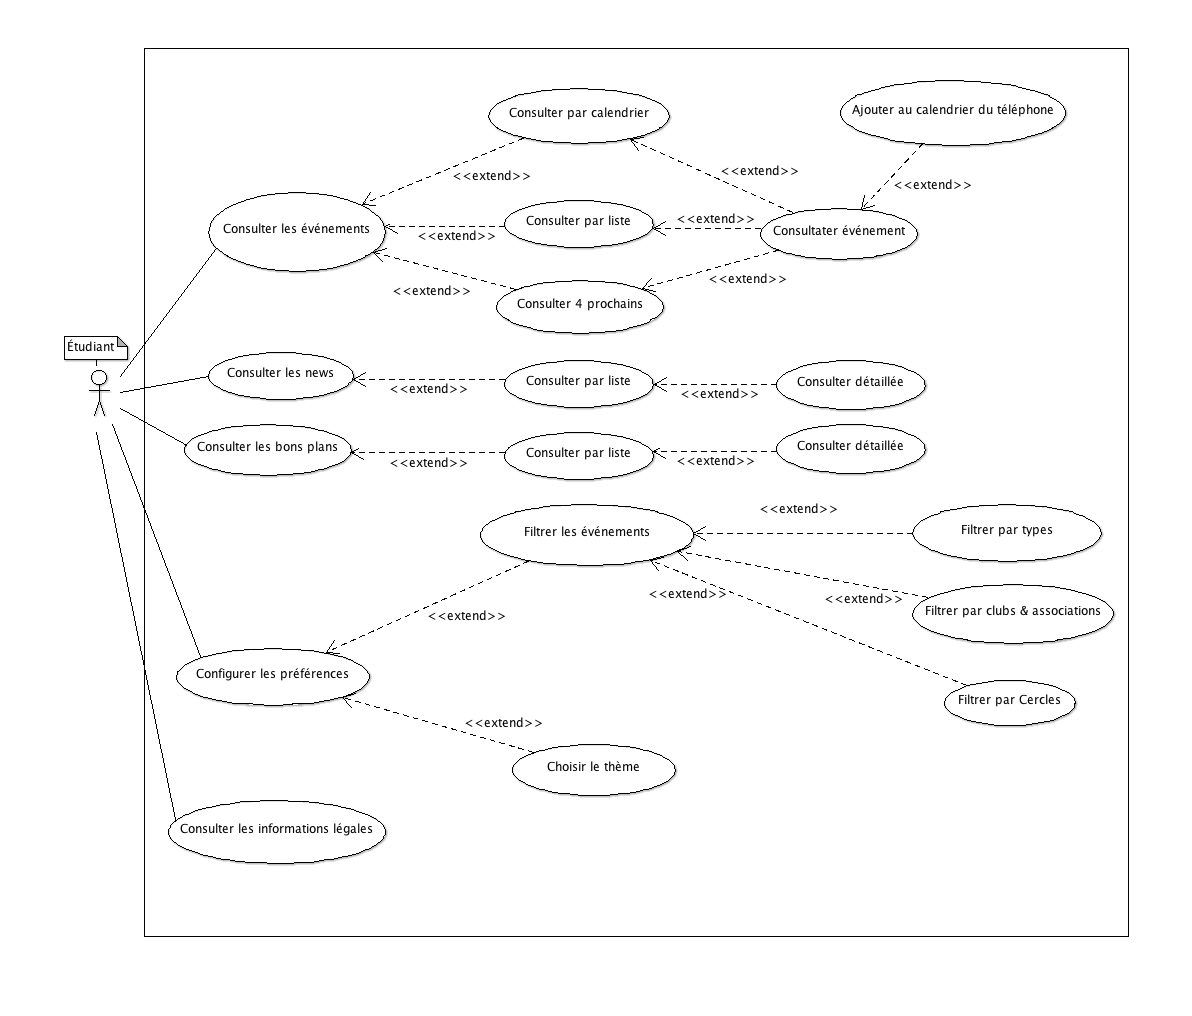
\includegraphics[width=20cm,height=15cm]{cas_utilisation.png}
\end{figure}

\newpage

\subsubsection{Modèle de tâches}
\vfill
\textbf{Fonctionnalités principales}
\begin{figure}[h!]
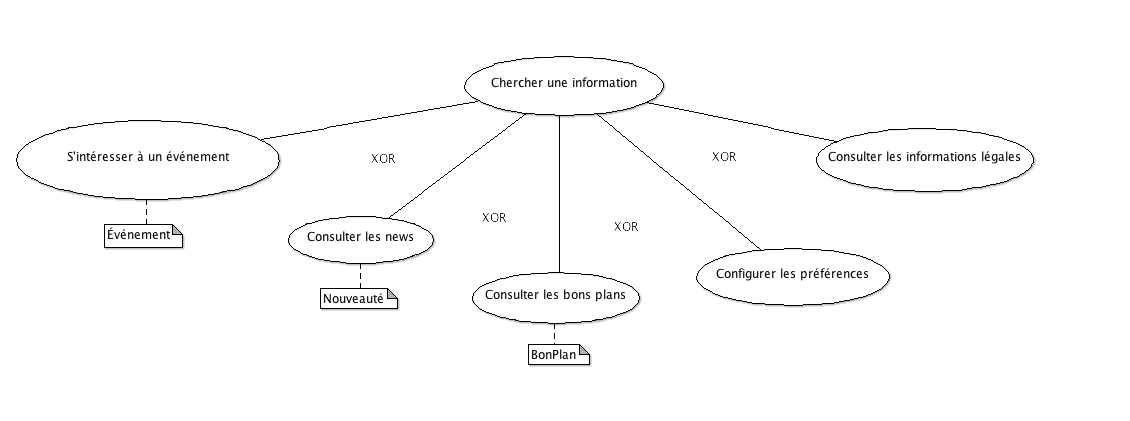
\includegraphics[width=18cm,height=6cm]{taches_generales.png}
\end{figure}

\textbf{S'intéresser à un événement}
\begin{figure}[h!]
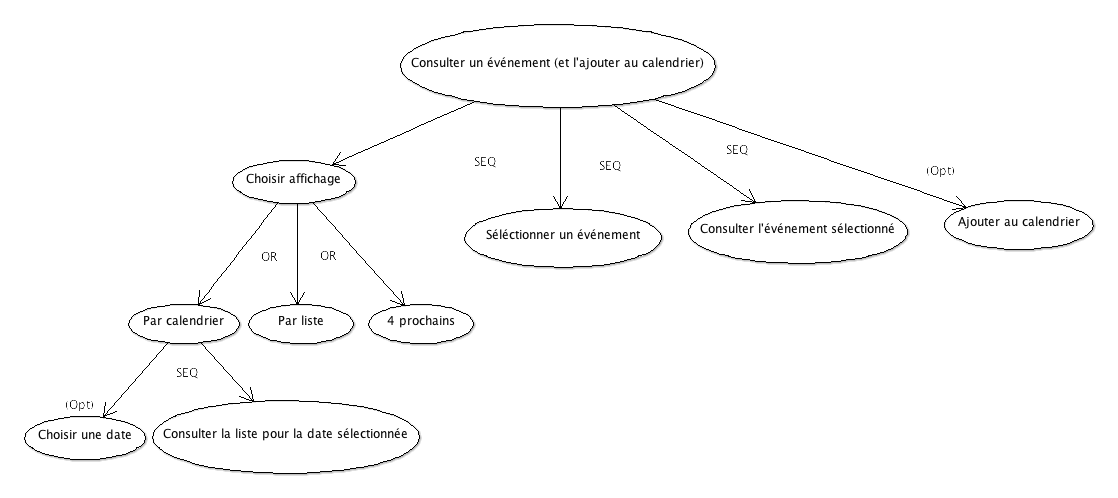
\includegraphics[width=18cm,height=11cm]{consulter_evenements.png}
\end{figure}
\vfill
\clearpage

\textbf{Consulter une news}
\vfill
\begin{figure}[h!]
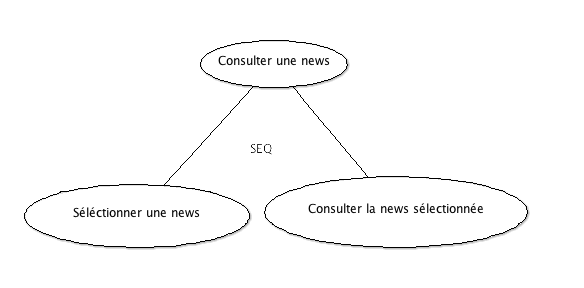
\includegraphics[width=18cm,height=8cm]{consulter_news.png}
\end{figure}

\textbf{Consulter un bon plan}

\begin{figure}[h!]
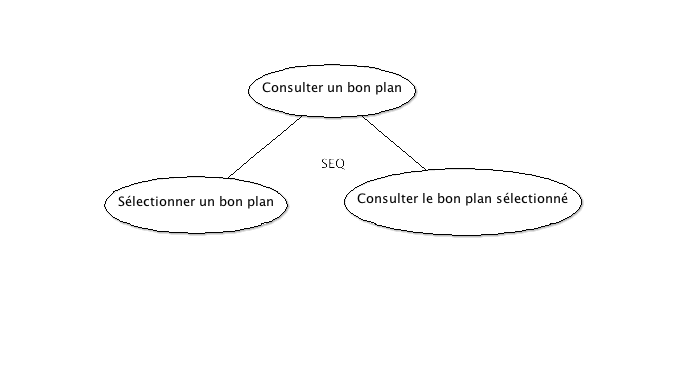
\includegraphics[width=18cm,height=8cm]{consulter_bonplans.png}
\end{figure}

\vfill
\clearpage
\vfil
\textbf{Configurer les préférences}
\begin{figure}[h]
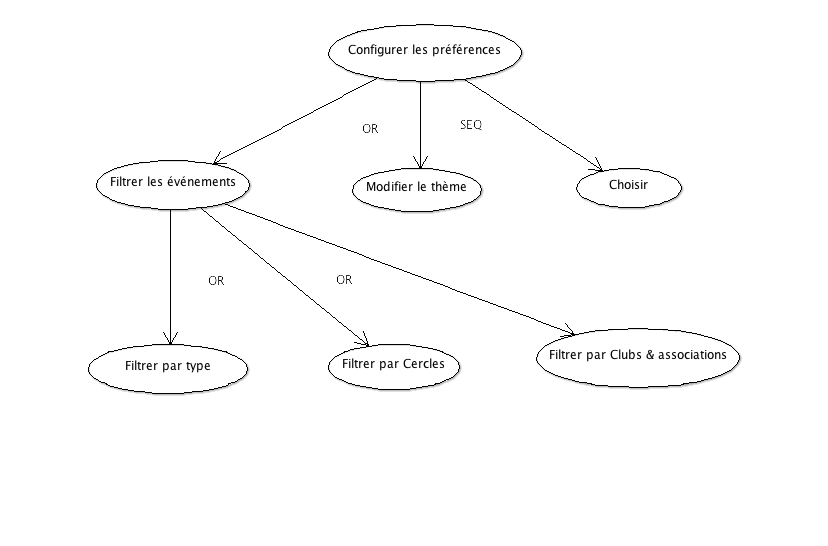
\includegraphics[width = \textwidth,height=8cm]{configurer_preferences.png}
\end{figure}
%%%%%% Fin DSE
\subsubsection{Modélisation UML}
Le diagramme suivant représente la modélisation objet du domaine d'application qui guide nos choix de conception.
\begin{figure}[h]
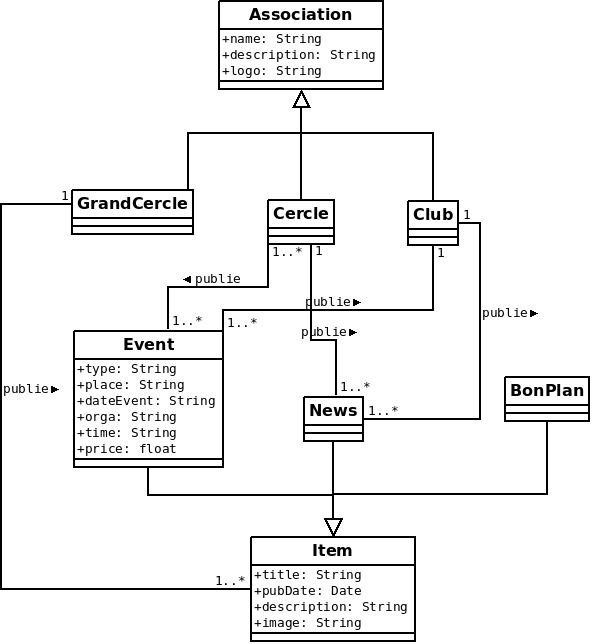
\includegraphics[width = 12cm,height=8cm]{classes.png}
\end{figure}

\vfill
\clearpage

\subsubsection{Sketching}
\textbf{Remarques générales}

L'affichage des événements se fait dans trois manières différentes : par calendrier, par liste et les quatre prochaines événements . Ces trois visualisations se trouvent sur des pages distinctes et le changement de page se fait par un mouvement de gauche a droit ou de droit a gauche du doit sur l'écran tactile. Un objet standard composé de 3 indicateurs circulaires permette d'informer l'utilisateur de la page courante et de signaler le changement.

Dans l'affichage calendrier, l'utilisateur peut accéder à la date qu'il souhaite pour voir les événements correspondants. Dans la liste se trouvent tous les événements prochaines à partir du jour présent.


\textbf{Sketching pour l'application iOS}

Pour l'application iOS, les affichages seront implémentés en utilisant les éléments par défaut d'Apple. L'avantage du point de vue de l'utilisateur est qu'il pourra naviguer facilement dans l'application comme il reconnaîtra les différentes objets.

\underline{Pages événements}

Dans l'affichage liste des événements (Fig. \ref{even_liste}) il y a les événements groupés par date, utilisant le tableau par sections d'iOS. 


\begin{figure}[htbp]
	\begin{minipage}[c]{.33\linewidth}
		\begin{center}
			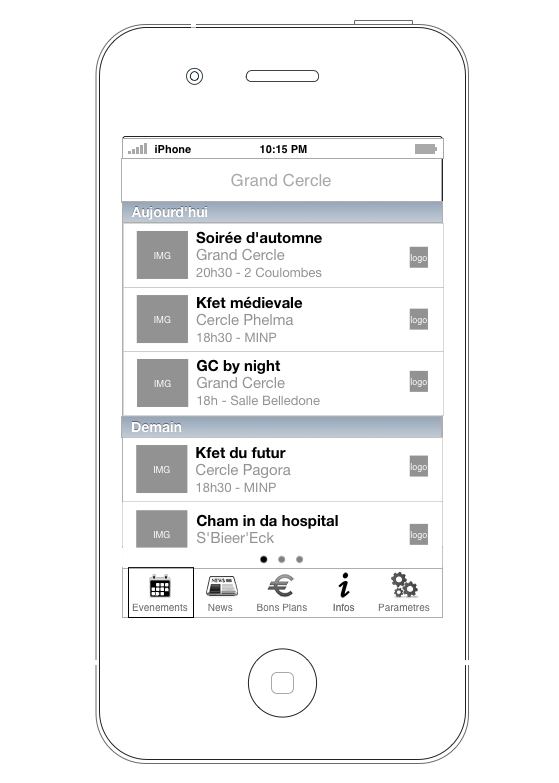
\includegraphics[scale=0.3]{../../Sketch/iOS/evenements_liste.png}
		\end{center}
	\caption{Calendrier}
	\label{calendar}

	\end{minipage}
	\hfill
	\begin{minipage}[c]{.33\linewidth}
		\begin{center}
			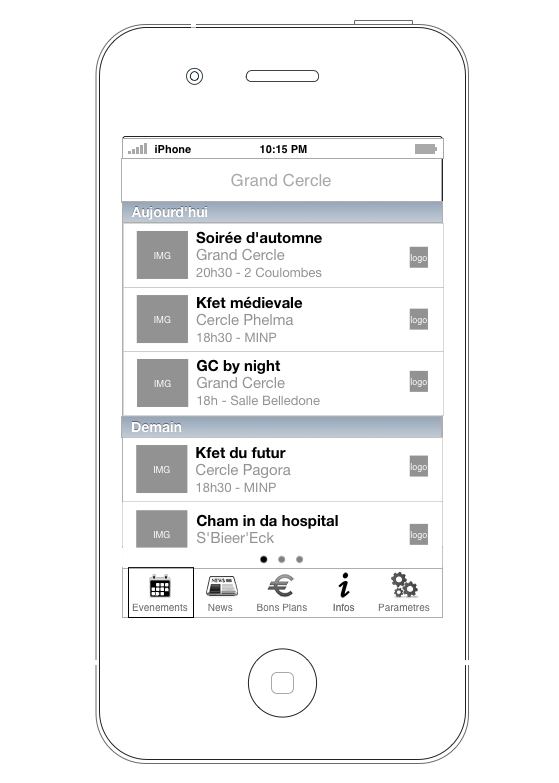
\includegraphics[scale=0.3]{../../Sketch/iOS/evenements_liste.png}
		\end{center}
	\caption{Liste}
	\label{even_liste}

	\end{minipage}
	\begin{minipage}[c]{.32\linewidth}
		\begin{center}
			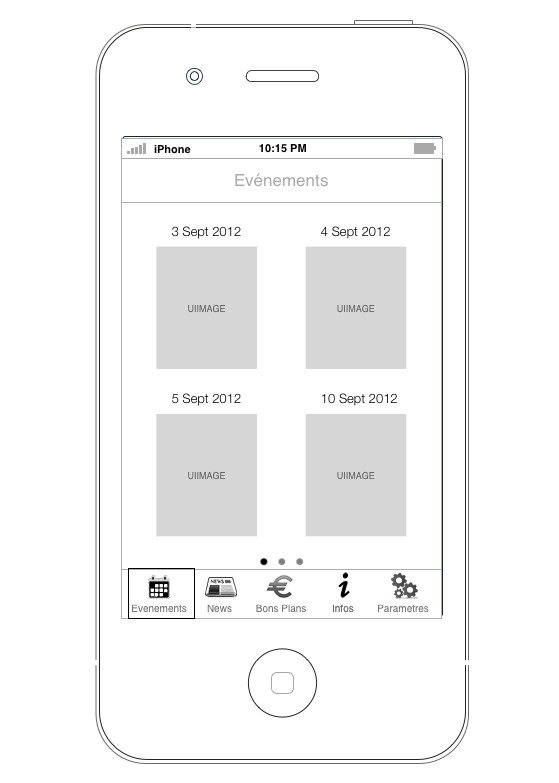
\includegraphics[scale=0.3]{../../Sketch/iOS/evenements_4_prochains.png}
		\end{center}
	\caption{4 prochains}
	\label{4_prochains}

	\end{minipage}
\end{figure}
\vfill
\clearpage

\begin{figure}[htbp]
	\begin{minipage}[c]{.50\linewidth}
		\begin{center}
			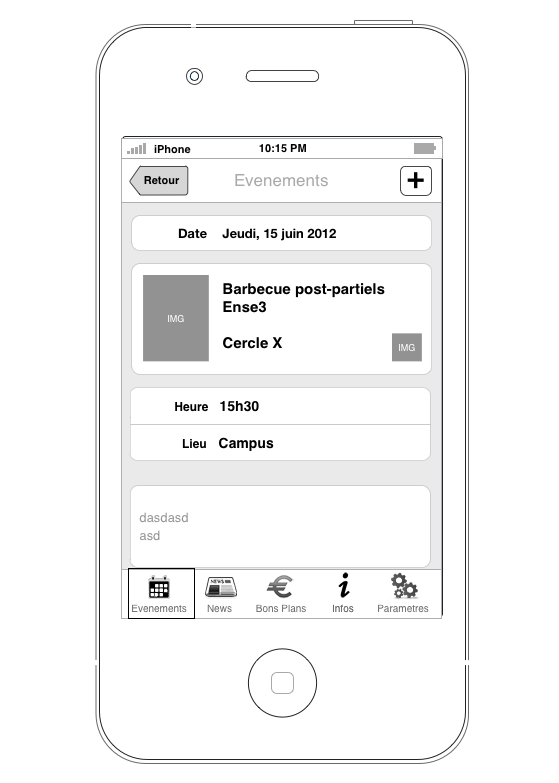
\includegraphics[scale=0.3]{../../Sketch/iOS/evenements_detail.png}
		\end{center}
	\caption{Détails d'un événement}
	\end{minipage}
	\hfill
	\begin{minipage}[c]{.50\linewidth}
		\begin{center}
			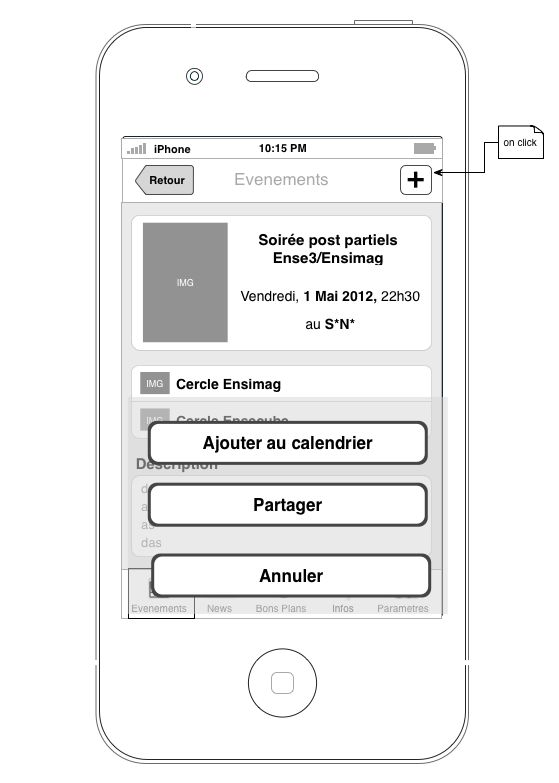
\includegraphics[scale=0.3]{../../Sketch/iOS/evenements_detail_plus.png}
		\end{center}
	\caption{Exporter événement}
	\end{minipage}
\end{figure}

Les sketch concernant les autres pages de l'application sont disponibles en annexe \ref{sketchiOS}.\\

\newpage

\textbf{Sketching pour l'application Android}

Les sketching de l'application Android ont été réalisés avec un plugin d'eclipse, \textbf{Wireframe Sketcher}, qui ne permet pas de séléctionner des onglets différents. Ainsi, dans toutes les pages présentées ci-après, l'onglet qui est mis en relief est toujours l'onglet "Evénements", ce qui ne représente pas toujours l'onglet actif. Afin de régler ce problème, l'onglet actif a été mis en gras.

\underline{Pages événements}
\vfill
\begin{figure}[htbp]
	\begin{minipage}[c]{.50\linewidth}
		\begin{center}
			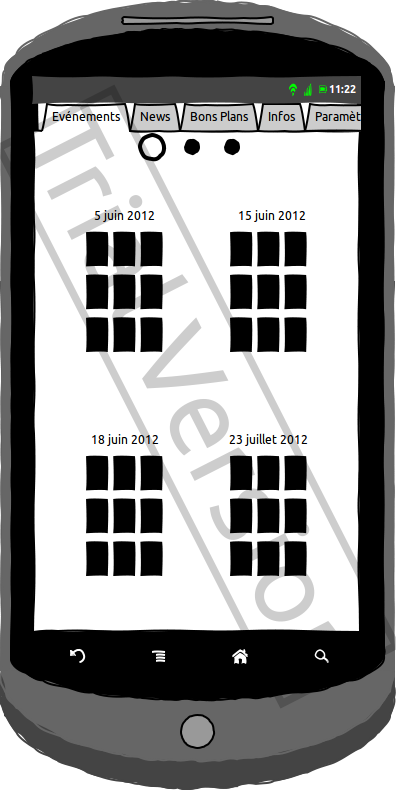
\includegraphics[scale=0.3]{../../Sketch/Android/quatreEvent.png}
		\end{center}
	\end{minipage}
	\hfill
	\begin{minipage}[c]{.50\linewidth}
		\begin{center}
			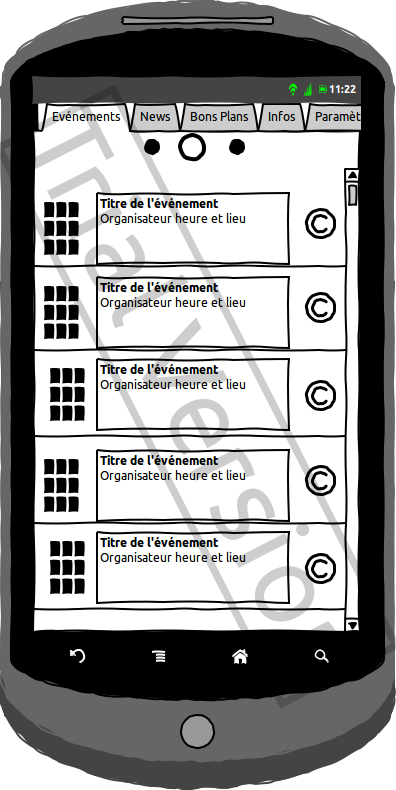
\includegraphics[scale=0.3]{../../Sketch/Android/ListEvent.png}
		\end{center}
	\end{minipage}
\end{figure}

\begin{figure}[htbp]
	\begin{minipage}[c]{.50\linewidth}
		\begin{center}
			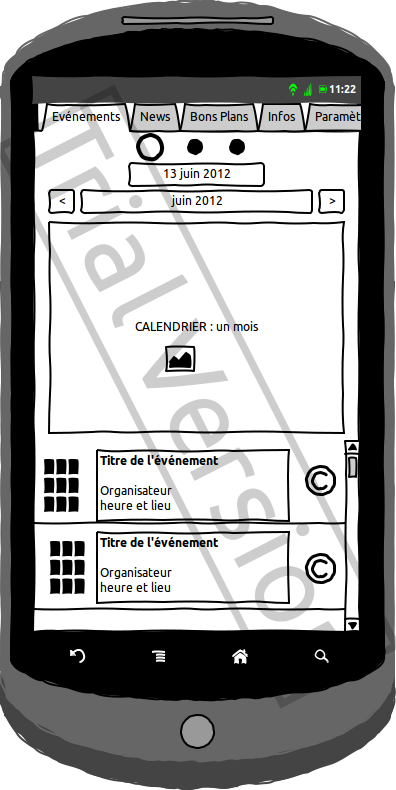
\includegraphics[scale=0.3]{../../Sketch/Android/Calendrier.png}
		\end{center}
	\end{minipage}
	\hfill
	\begin{minipage}[c]{.50\linewidth}
		\begin{center}
			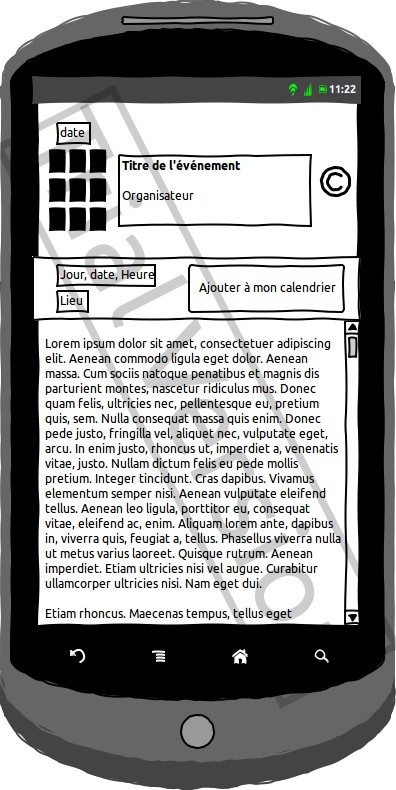
\includegraphics[scale=0.3]{../../Sketch/Android/DescrEvent.png}
		\end{center}
	\end{minipage}
\end{figure}
Les sketch concernant les autres pages de l'application sont disponibles en annexe \ref{sketchAndroid}.
\vfill
\clearpage





\subsection{Conception logicielle}

\subsubsection{Architecture logicielle}
L'architecture utilisé pour les deux applications est l'architecture Modèle-Vue-Contrôleur qui à été facilement mise en œuvre avec les frameworks Android pour Java et Cocoa Touch pour Objective-C.

L'application réalisée ne peut existée sans que le site du Grand Cercle ne soit tenu à jour. Nous récupérons ainsi toutes les données présentes sur ce site à l'aide de cinq parsers qui agissent sur cinq fichiers xml différents en même temps que l'affichage d'accueil à l'aide de threads.\\

\noindent Plusieurs choses sont ainsi réalisées lors de cette phase:
\begin{itemize}
\item récupération des données sur le site
\item création des listes de clubs, de cercles et de types d'événements, nécessaire pour la gestion des préférences.
\item initialisation de toutes les autres structures de données (listes des données relatives aux événements, aux news, aux bons plans).
\item initialisation des préférences (dictionnaire pour iOS et base de donnée pour Android)
\end{itemize}

\vspace{0.5cm}
\noindent Un des points importants de la récupération de donnée est la présence ou non de connexion internet: 
\begin{itemize}
\item soit une connexion internet est disponible. Dans ce cas on sauvegarde les fichiers xml en provenance du site dans la mémoire et on parse ces fichiers qui sont alors contenues dans la mémoire interne du téléphone.
\item soit aucune connexion n'est possible et dans ce cas, on parse les données qui sont dans la mémoire, sauvegardées lors de connexions antérieures.
\end{itemize}

\noindent Lors de la première utilisation de l'application, un message est affiché à l'utilisateur s'il n'est pas connecté à internet pour lui indiquer qu'aucune donnée n'a pu être chargée (mais l'application se lance correctement).
 Lors de l'initialisation de la base de données, aucun filtre n'est appliqué et les données sont récupérées dans leur totalité, l'utilisateur ayant ensuite le choix d'appliquer ou non ces filtres.

\subsubsection{iOS}
Pour Objective-C, les classes sont séparées dans les fichiers header (extension \texttt{.h}) et les fichiers d'implémentation (extension \texttt{.m})
Les classes qui correspondent au modèle contiennent les attributs et les mutateurs comme dans le modèle objet présenté dans la figure \ref{modele_objet}. Les classes de la vue sont les fichiers avec l'extension \texttt{.xib} qui sont des fichiers de type \texttt{xml}. Ces fichiers peuvent être crées et édités facilement grâce à l'interface graphique fournie par Xcode. Tous les vues sont contrôlés par des classes \texttt{ViewController} qui font la connexion entre les objets et les données des contrôleurs.
Les classes du contrôleur sont les classes pour récupérer, parser et filtrer les données.\\

{\bf Patrons de conception}

Pour toutes les classes contrôleur nous avons utilisé le \texttt{Singleton} pour s'assurer d'avoir une seule instance qui effectue les traitements des données.


Nous avons utilisé aussi quelques autres patrons de conception fournis par le framework et par Xcode. \\
\begin{itemize}
	\item {\bf Composite} est le patron utilisé pour la hiérarchie des éléments de la vue. Chaque élément est une sous-classe de \texttt{UIView} donc il hérite tous ses méthodes.
En utilisant l'interface graphique, nous avons ajouté des objets à la vue en suivant une hiérarchie\\
	\item {\bf Commande} est le patron utilisé pour rédiger l'exécution quand un événement apparaît. Cela à été fait toujours à l'aide de l'interface graphique, en reliant un objet avec une méthode.\\
	\item {\bf Observateur} est le patron qui fournit la mise à jour facile entre les vues et les modèles. Nous avons utilisé \texttt{Notification Center} pour informer la vue des changements du modèle et vice-versa.
\end{itemize}



\subsubsection{Android}
La technologie Android repose sur la dualité entre la langage \texttt{Java} et le langage \texttt{xml}. A chaque affichage correspond un fichier \texttt{xml} qui met en place les différentes fenêtres qui constituent l'écran, appelées des \og layouts \fg, ainsi qu'un fichier Java qui représente ce qu'on appelle une activité, c'est à dire la fenêtre visible à l'écran. La vue offerte à l'utilisateur est mise en place par la méthode setContentView([fichier xml]). Néanmoins, ce fichier xml en paramètre de la méthode mentionnée correspond à une configuration statique de l'affichage. Ainsi, dès que nous avons besoin de modifier dynamiquement une vue, nous le faisons dans le code Java, grâce à l'identifiant de la vue considérée renseigné dans le code xml : c'est ce qui fait la dualité Java/xml. \'Etant donné que le positionnement des différents objets dans les layouts est moins facile en Java que dans un fichier xml, il est avantageux d'utiliser le xml dès que cela est possible.

{\bf Patrons de conception}

\begin{itemize}
	\item {\bf Singleton} a été mis en œuvre pour notre base de donnée, afin de s'assurer qu'elle n'est instanciée qu'une seule fois et ainsi d'assurer un traitement des données cohérent pour toute l'application.\\
	\item {\bf Commande} est le patron utilisé pour rédiger l'exécution quand un événement apparaît (exemple : appuie sur une zone de l'écran, sur un bouton, \dots)\\
	\item {\bf Observateur} est utilisé lorsque les préférences sont modifiées par l'utilisateur. Il se résume a un seul appel à la méthode \texttt{ParseEvent()} afin d'actualiser les données affichée et stockées, étant donné que les données qui ne correspondent pas aux préférences n'ont pas de raison d'être stockées dans les structures de données appropriées.
	\item {\bf Fabrique} est nécéssaire pour construire une instance du parser SAX qui permet de récupérer les données.
\end{itemize}
Dans l'application Android, nous avons préféré utilisé un parser SAX plutôt qu'un DOM, puisque le SAX est plus rapide que le DOM (cf \href{http://www.developer.com/ws/android/development-tools/Android-XML-Parser-Performance-3824221-2.htm}{http://www.developer.com/ws/android/development-tools/Android-XML-Parser-Performance-3824221-2.htm}).



Notre application témoigne d'une volonté de simplicité et de rapidité auprès des utilisateurs. Ainsi, la classe \texttt{DragableSpace.java} permet de \og slider \fg afin de limiter le nombre d'onglets. Le changement de vue n'est réalisé que si l'utilisateur effectue le slide assez rapidement.

\section{Mise en œuvre}

\subsection{iOS}
{\bf Parser}
Nous avons utilisé un thread pour parser les informations de l'\texttt{XML} pour ne pas bloquer l'interface utilisateur. Quand l'information est disponible une notification est envoyé et la mise à jour de l'affichage est faite.


{\bf Préférences}

Pour sauvegarder les préférences nous avons utilisé le dictionnaire par défaut de l'application 
\texttt{[NSUserDefaults standardUserDefaults]}. A la clé choisie il y q un pointer vers l'objet qui est un dictionnaire pour les filtres et un vecteur pour la choix de thème. Pour le filtre de cercle, club et type nous avons un dictionnaire des booléens où la clé est le nom du cercle, du club ou le type. La couleur de la thème est sauvegardé en RGB dans un vecteur de taille 3. 
 
{\bf Cache des images}

Chaque fois quand on trouve une nouvelle image à télécharger, on la met dans une queue et quand elle est disponible elle va être sauvegardé dans la mémoire. On garde un dictionnaire ayant comme clé le hash de l'URL de l'image. Le téléchargement est fait dans un thread et une notification est envoyé pour mettre à jour l'affichage.

{\bf Librairies externes}

Pour parser l'information provenant du fichier \texttt{XML} nous avons utilisé la librairie \texttt{TBXML} qui d'après les critiques est le plus rapide et le plus adapté a nos besoins. De plus, une classe avec des extensions pour \texttt{NSString} est utilisé pour décoder les entités \texttt{HTML}\\
\indent On se sert de la librairie \texttt{tapuku} pour la gestion du cache des images et pour le calendrier. Des changements ont étés fait au calendrier pour factoriser le code et pouvoir contrôler la taille du calendrier facilement.
Une simple classe appellé \texttt{Reachability} offre les fonctionnalités pour tester la connexion internet de l'utilisateur et d'agir en conséquence.


\subsection{Android}
{\bf Parser}
Nous avons utilisé un thread pour parser les informations de l'\texttt{XML} pour ne pas bloquer l'interface utilisateur. Quand les cinq parser ont terminé leur execution, la méthode \texttt{onPostExecute(Void result)} est appelée, et crée la classe \texttt{GCM}. La différence avec les autres activités est que \texttt{GCM} étend la classe \texttt{TabActivity} et non \texttt{Activity}. En effet, cette activité permet de construire les onglets de notre application à l'aide d'un objet appelé \texttt{TabHost}. Toutes les vues des différents onglets sont crées dans GCM.java, ce qui permet à l'utilisateur de naviguer rapidement entre les différents onglets.


{\bf Préférences}
Pour sauvegarder les préférences, une base de donnée \texttt{SQLite} a été employée. Chaque préférence (par cercle, par club, par type et le thème) est stockée dans une table différente.
 
{\bf Cache des images}

A chaque image trouvée par le parser, on associe une clé de type \texttt{String} qui est en fait l'url de l'image. On stocke ensuite dans une \texttt{HashMap} le fichier bitmap correspondant à cette clé.\\
Deux conventions ont été adoptée pour le stockage des images :
\begin{itemize}
\item soit l'image est une affiche d'événement et elle est stockée dans le cache pendant une semaine
\item soit l'image est un logo d'association ou d'enseigne (pour les bons plans) et elle est stockée de manière infinie dans le cache\\
\end{itemize}

{\bf Librairies externes}

Afin de pourvoir réaliser la fonctionnalité d'import d'un événement au calendrier du téléphone, nous avons été obligé d'ajouter à nos options de compilation la librairie \texttt{android-8}, issue de l'API 8 d'Android. Notre application doit fonctionner sur les téléphones équipés des API 7 et plus, donc cette librairie est inclue dans les API 8 et plus, mais posait un problème pour l'API 7. Nous l'avons donc rajouté lors de la compilation, et elle fonctionne sur l'API 7 (téléphones sous Android 2.1).


\section{Validation}
Les deux applications ont été validées suivant une démarche commune afin d'assurer un niveau de qualité équivalent d'une application à l'autre.

Certains tests ont été réalisés au fur et à mesure du développement des applications, d'autres ont été effectués sur des prototypes fonctionnels et enfin la version finale des deux application a été évaluée par un panel d'utilisateurs potentiels.

\subsection{Tests unitaires}
Chaque module a été testé grâce à des tests unitaires. Majoritairement, ces tests consistent à envoyer en entrée du module un cas de test spécifique, de tracer le module afin de vérifier qu'au cours de l’exécution rien d'anormal ne se produit, et de récupérer en sortie un résultat que l'on compare au résultat attendu. Les tests spécifiques sont pour la plupart des tests dits "boite blanche".

Ces tests sont avant tout des tests techniques qui permettent de s'assurer qu'il n'y a pas d'erreur d'analyse et/ou de programmation.

\subsection{Tests d'intégration et de validation informatique}
Ces tests permettent de tester la cohérence et l'articulation des modules entre eux, de vérifier que les modules communiquent bien entre eux.


Ces tests ont été réalisés de manière similaire aux tests unitaires, à savoir un traçage des opérations effectuées et une comparaison du résultat obtenu avec le résultat attendu.

\subsection{Validation ergonomique}
Afin de vérifier la conformité de nos différents prototypes avec les besoins formulés par les utilisateurs, regroupés dans le cahier des charges, nous avons fait appel à un panel d'utilisateurs potentiels disposant de leur propre smartphone sous iOS ou Android, et ce dans le but de confronter ces applications à des utilisateurs habitués aux pratiques sur ces deux systèmes d'exploitation.\\

Nous avons mis en place des une procédure qui nous a permis de toujours demander à ces utilisateurs potentiels d'effectuer les mêmes manipulations dans l'application et d'observer leur réactions. Pour prendre en compte leurs remarques et ne pas en oublier, nous avons procédé à des enregistrements vidéo de ces tests.\\
Pour enrichir l'application, nous avons créé une URL de test sur le site du \texttt{Grand Cercle} afin de faire afficher un grand nombre d'événements dans l'application et de rendre le test plus réaliste.\\

Le protocole est fourni en annexe \ref{protocole}, il reprend la totalité des fonctionnalités implémentée dans notre application, et comprend des manipulations très simple pour commencer ainsi que des tâches jugées plus difficile à réaliser pour finir.


\appendix
\addappheadtotoc

\newpage

\section{Sketching pour l'application iOS}
\label{sketchiOS}
\underline{Pages news}
\begin{figure}[h!]
	\begin{minipage}[c]{.50\linewidth}
		\begin{center}
			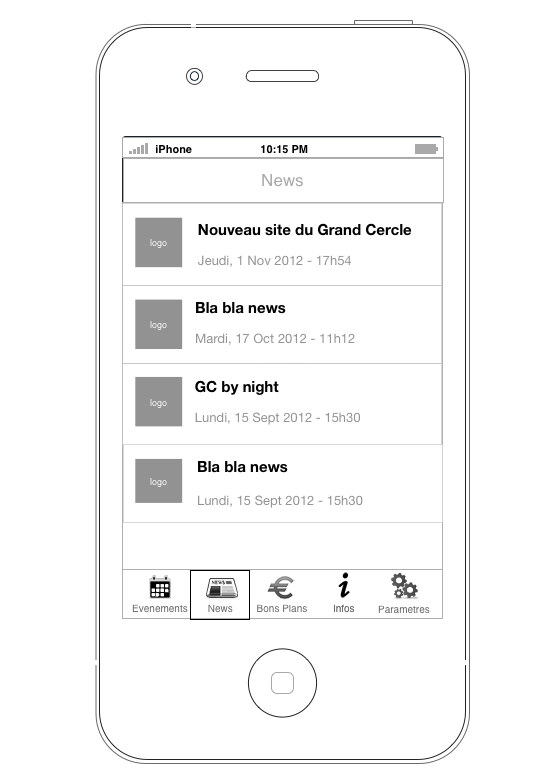
\includegraphics[scale=0.3]{../../Sketch/iOS/news_liste.png}
		\end{center}
	\caption{Liste de news}

	\end{minipage}
	\hfill
	\begin{minipage}[c]{.50\linewidth}
		\begin{center}
			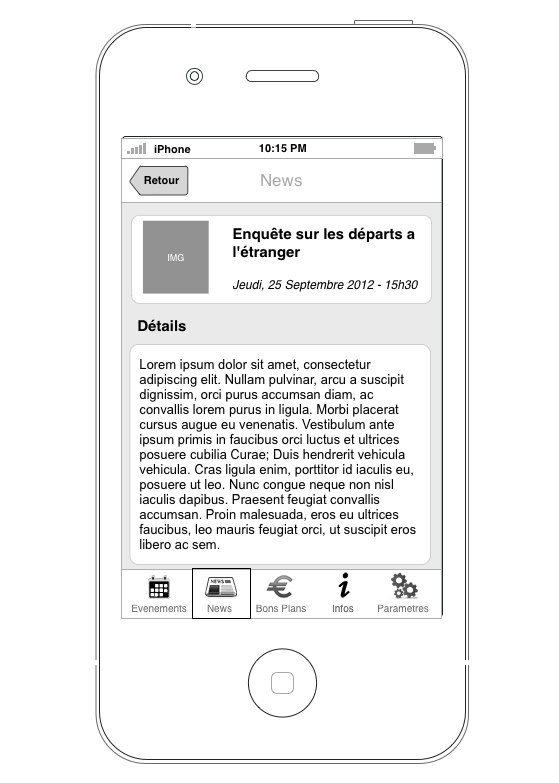
\includegraphics[scale=0.3]{../../Sketch/iOS/news_detail.png}
		\end{center}
	\caption{Détails d'un news}
	\end{minipage}
\end{figure}
\vfill
\clearpage
\underline{Pages bons plans}
\begin{figure}[htbp]
	\begin{minipage}[c]{.50\linewidth}
		\begin{center}
			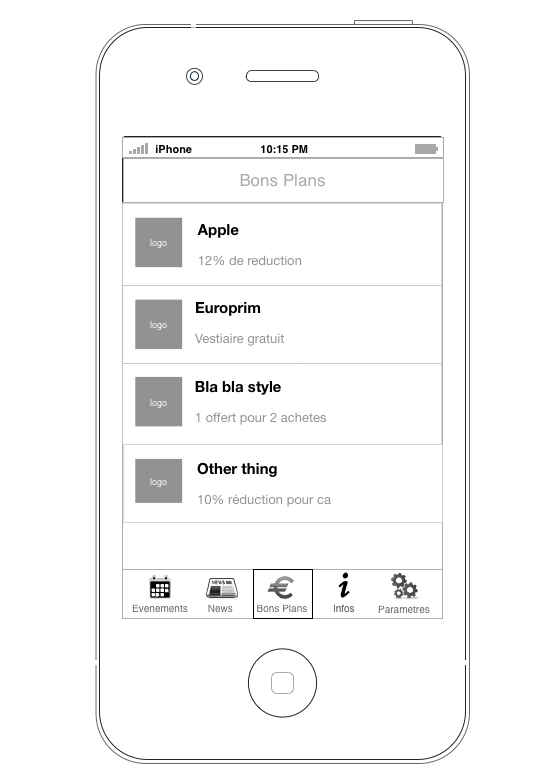
\includegraphics[scale=0.29]{../../Sketch/iOS/bons_plans_liste.png}
		\end{center}
	\caption{Liste de bons plans}

	\end{minipage}
	\hfill
	\begin{minipage}[c]{.50\linewidth}
		\begin{center}
			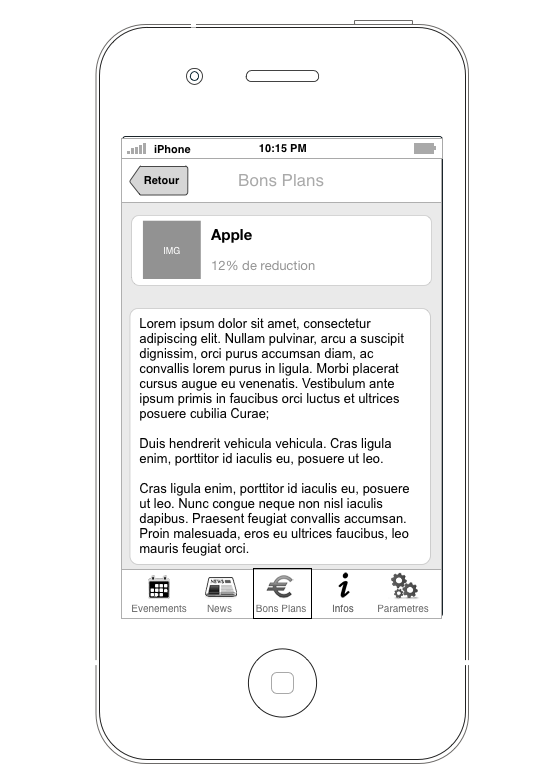
\includegraphics[scale=0.29]{../../Sketch/iOS/bons_plans_detail.png}
		\end{center}
	\caption{Détails d'un bon plan}

	\end{minipage}
\end{figure}

\underline{Page informations}
\begin{figure}[h!]
	\begin{minipage}[c]{.50\linewidth}
		\begin{center}
			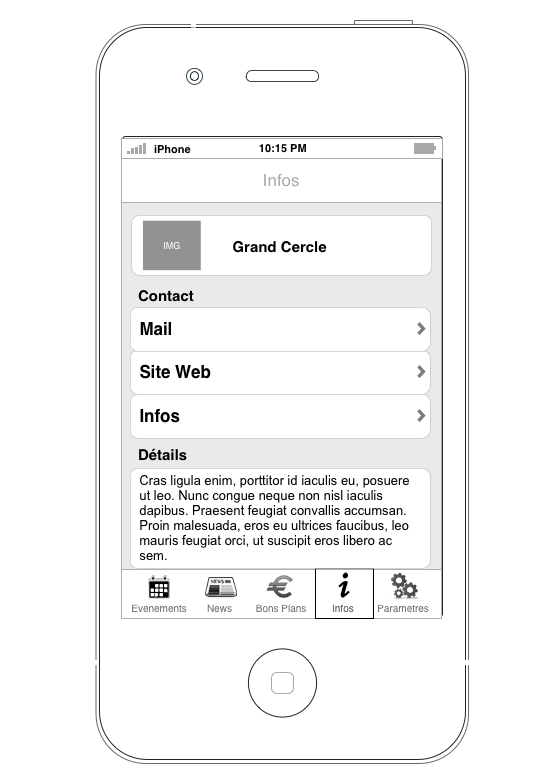
\includegraphics[scale=0.29]{../../Sketch/iOS/infos.png}
		\end{center}
	\caption{Page d'informations}
	\end{minipage}
\end{figure}

\clearpage
\underline{Pages paramètres}

En ce qui concerne les préférences utilisateurs, tous les choix se feront par le biais de checkbox comme pour l'application Android mais il n'y aura pas de bouton pour valider les choix effectués par les utilisateurs. 
En effet, les choix de thème seront pris en compte immédiatement après le "check" et les choix de filtre seront pris en compte quand l'utilisateur sortira de la page courante où il formule ses choix.
\begin{figure}[htbp]
	\begin{minipage}[c]{.50\linewidth}
		\begin{center}
			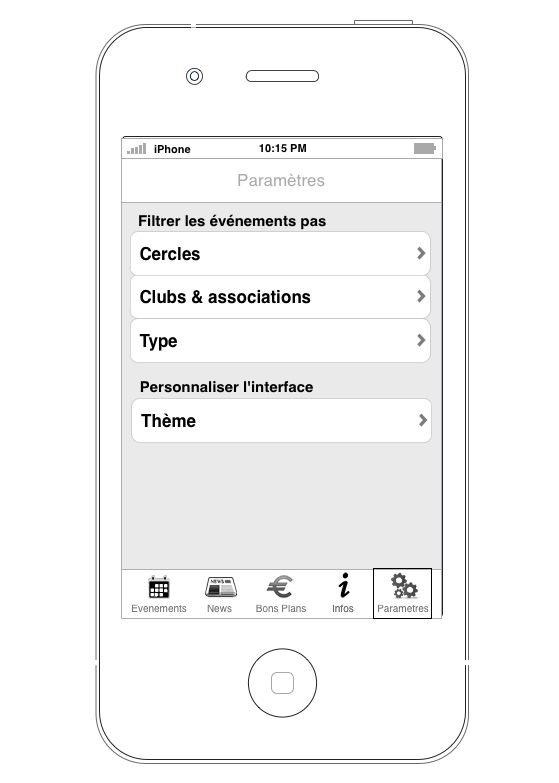
\includegraphics[scale=0.3]{../../Sketch/iOS/parametres.png}
		\end{center}
	\end{minipage}
	\hfill
	\begin{minipage}[c]{.50\linewidth}
		\begin{center}
			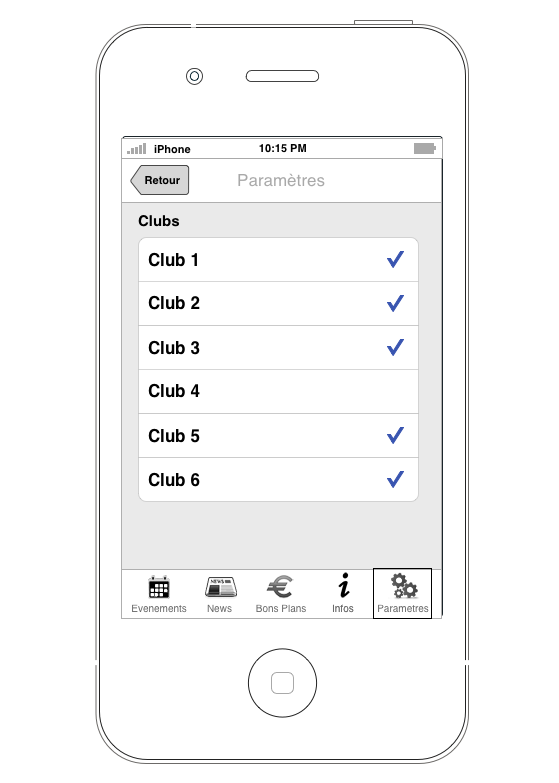
\includegraphics[scale=0.3]{../../Sketch/iOS/parametres_detail.png}
		\end{center}
	\end{minipage}
\end{figure}
\vfill
\clearpage

\section{Sketching pour l'applicationAndroid}
\label{sketchAndroid}
\underline{Pages news}\\
Dans cette section, l'onglet actif est l'onglet "News".
\vfill
\begin{figure}[htbp]
	\begin{minipage}[c]{.50\linewidth}
		\begin{center}
			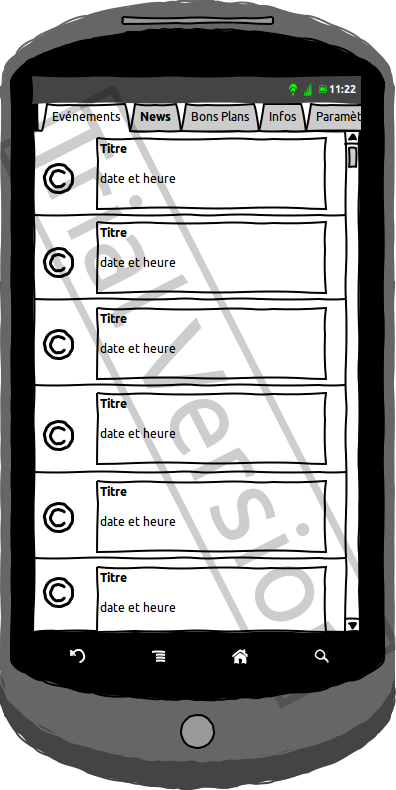
\includegraphics[scale=0.3]{../../Sketch/Android/News.png}
		\end{center}
	\end{minipage}
	\hfill
	\begin{minipage}[c]{.50\linewidth}
		\begin{center}
			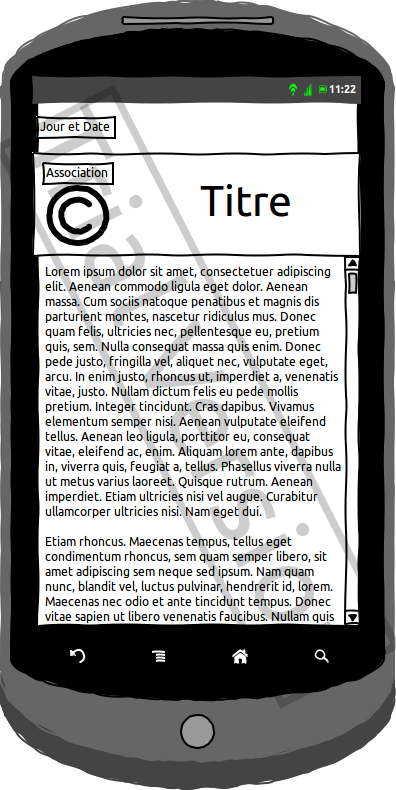
\includegraphics[scale=0.3]{../../Sketch/Android/DescrNews.png}
		\end{center}
	\end{minipage}
\end{figure}

\underline{Pages bons plans}\\
Dans cette section, l'onglet actif est l'onglet "Bons plans".
\begin{figure}[htbp]
	\begin{minipage}[c]{.50\linewidth}
		\begin{center}
			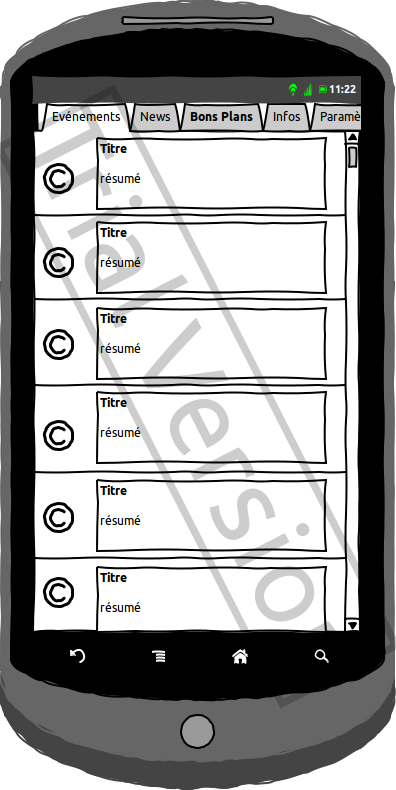
\includegraphics[scale=0.3]{../../Sketch/Android/BP.png}
		\end{center}
	\end{minipage}
	\hfill
	\begin{minipage}[c]{.50\linewidth}
		\begin{center}
			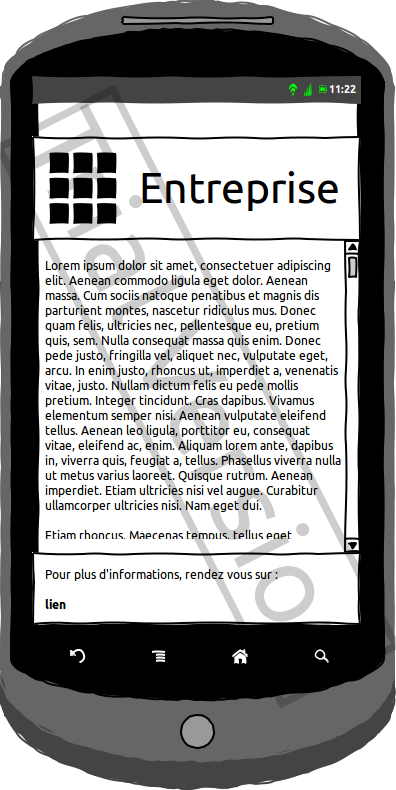
\includegraphics[scale=0.3]{../../Sketch/Android/DescrBP.png}
		\end{center}
	\end{minipage}
\end{figure}
\vfill
\clearpage

\underline{Page informations}\\
Dans cette section, l'onglet actif est l'onglet "Infos".
La page information présente sur la même page deux liens cliquables et une description du Grand Cercle de Grenoble INP.
\vfill
\begin{figure}[htbp]
	\begin{minipage}[c]{.50\linewidth}
		\begin{center}
			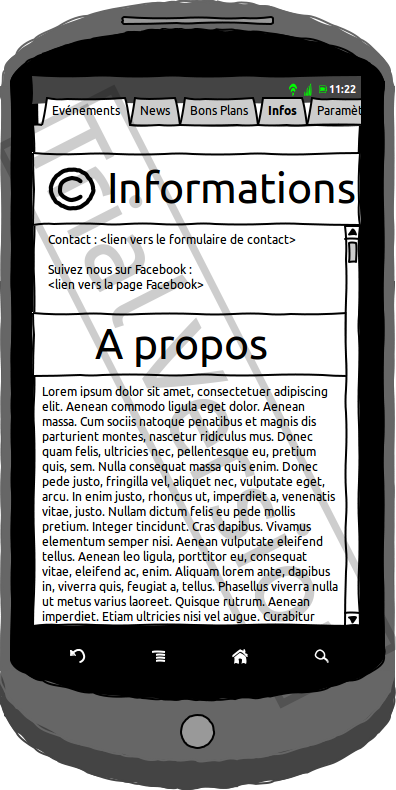
\includegraphics[scale=0.3]{../../Sketch/Android/Infos.png}
		\end{center}
	\end{minipage}
\end{figure}

\underline{Pages paramètres}\\
Dans cette section, l'onglet actif est l'onglet "Paramètres". 
Pour sauvegarder ses préférences, il est nécessaire d'appuyer sur le bouton "OK" avant de quitter la fenêtre. La sauvegarde est effectuée au moment de l'appui sur ce bouton
\begin{figure}[htbp]
	\begin{minipage}[c]{.33\linewidth}
		\begin{center}
			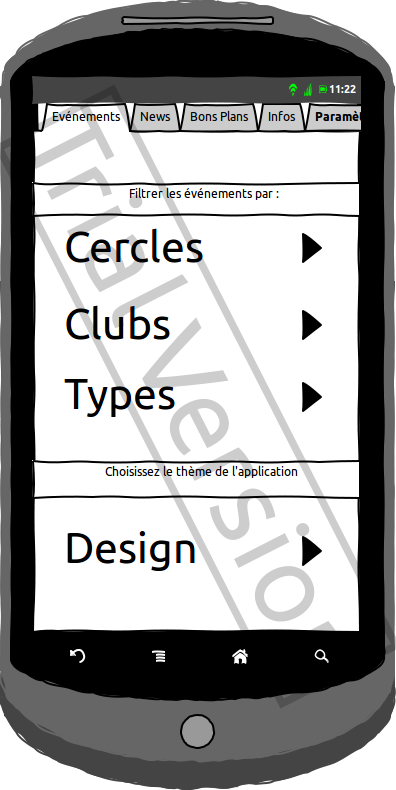
\includegraphics[scale=0.3]{../../Sketch/Android/Param.png}
		\end{center}
	\end{minipage}
	\hfill
	\begin{minipage}[c]{.33\linewidth}
		\begin{center}
			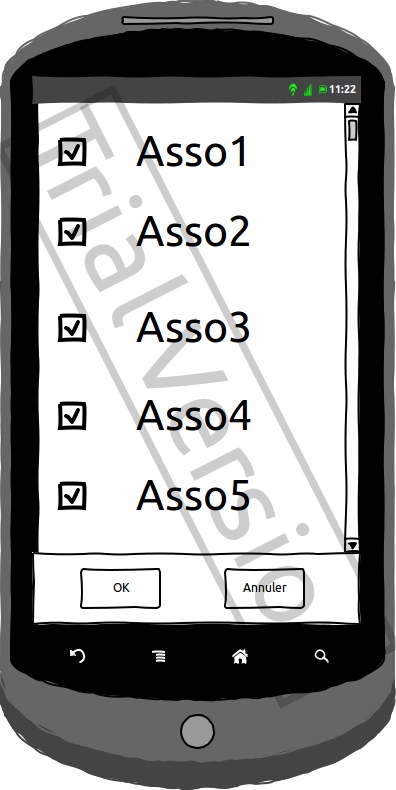
\includegraphics[scale=0.3]{../../Sketch/Android/Filtre.png}
		\end{center}
	\end{minipage}
	\hfill
	\begin{minipage}[c]{.32\linewidth}
		\begin{center}
			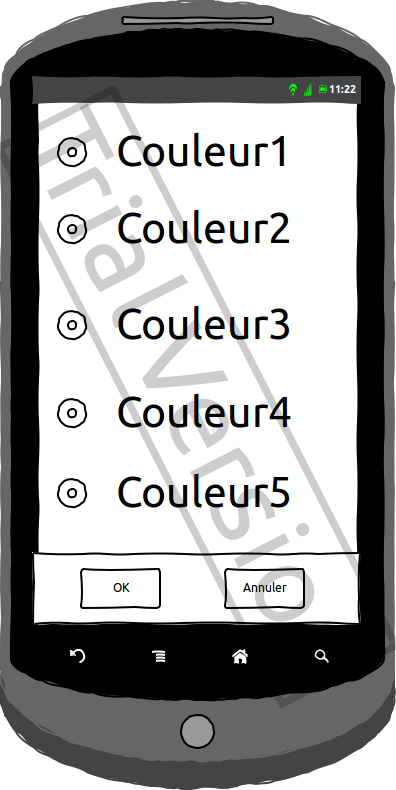
\includegraphics[scale=0.3]{../../Sketch/Android/Design.png}
		\end{center}
	\end{minipage}
\end{figure}
\vfill
\clearpage

\section{Protocole de tests utilisés dans les tests utilisateurs}
\label{protocole}

\textbf{1}. Lance l’application Grand Cercle Mobile.	
\\

\textbf{2}. Dis moi quels sont les 4 prochains événements qui se dérouleront  à Grenoble INP.	
\\

\textbf{3}. Donne moi les informations suivantes sur les 2 prochains événements : date, association qui organise, lieu, heure, type d’événement.
  \\

\textbf{4}. Y a-t-il un événement le 15 Novembre ?
  \\

\textbf{5}. Trouves un jour en Novembre où il y a un événement ?	
  \\

\textbf{6}. Trouve l’événement le plus éloigné en date ?	
  \\

\textbf{7}. Ajoute le au calendrier de ton téléphone	
\\

\textbf{8}. Imaginons que tu sois intéressé(e) par les événements de ton cercle et les Kfet de toutes les autres associations, fais en sorte d’afficher seulement les événements qui t’intéresse.
\\

\textbf{9}. Quelles sont les dernières nouvelles concernant les élus étudiants ?	
  \\

\textbf{10}.  Quand a été publié la dernière nouveauté concernant le Grand Cercle ?	
\\

\textbf{11}.  Cite moi trois enseignes dans lesquelles tu peux bénéficier de réductions en tant qu' étudiant de Grenoble INP.
  \\

\textbf{12}. Quelles sont les offres concernant la Fnac ?	
\\

\textbf{13}.  Trouve moi le lien de la page internet contenant les contacts du Grand Cercle.	
  \\

\textbf{14}.  Configure l’application aux couleurs de ton école ?	
\\

\textbf{15}. As tu des remarques, des choses à dire concernant l’application ?	
  



\end{document}
